%Le plan de recherche est à soumettre aux membres du jury et à l'EDPY au plus tard deux semaines avant l'examen.
%La page de couverture dûment signée par le doctorant et le directeur de thèse (et co-directeur si applicable)
%doit être soumise à l’EDPY au plus tard le jour de l'examen.
%The research plan shall be submitted to the jury members and EDPY at the latest two weeks before the candidacy exam.
%The cover page duly signed by the PhD student and the thesis advisor (and co-advisor if applicable) shall be submitted 
%to EDPY at the latest on the day of the exam.

\documentclass[11pt,titlepage]{article}

\usepackage[french,american]{babel}
\usepackage[utf8]{inputenc}
\usepackage[T1]{fontenc}
\usepackage{lmodern}
\usepackage{amsmath,amsfonts,amssymb}
\usepackage{graphicx}
\usepackage{geometry}                % See geometry.pdf to learn the layout options. There are lots.
\geometry{letterpaper}                   % ... or a4paper or a5paper or ... 
%\geometry{landscape}                % Activate for for rotated page geometry
%\usepackage[parfill]{parskip}    % Activate to begin paragraphs with an empty line rather than an indent
\usepackage{graphicx}
\usepackage{amssymb}
\usepackage{epstopdf}
\usepackage{color}
\usepackage[tt]{titlepic}
\usepackage{fancyhdr}
\usepackage{float}
\usepackage{caption}
\usepackage{subcaption}
\usepackage[bottom]{footmisc}
\usepackage{cite}
\usepackage{pdfpages}
\usepackage{braket}
\usepackage{lipsum}
\usepackage{amsmath,amsfonts}
\usepackage{listings}
\usepackage{float}
\usepackage{amsthm}
\usepackage{graphicx}
\usepackage{bm}
\usepackage{algorithm}
\usepackage{algpseudocode}
%\newtheorem{remark}{Remark}
\newtheorem{theorem}{Theorem}
\newtheorem{assumption}{Assumption}
\newtheorem{definition}{Definition}
\newtheorem{proposition}{Proposition}
\newtheorem{corollary}{Corollary}
\usepackage{color} %red, green, blue, yellow, cyan, magenta, black, white
\definecolor{mygreen}{RGB}{28,172,0} % color values Red, Green, Blue
\definecolor{mylilas}{RGB}{170,55,241}
\usepackage{xargs}                      % Use more than one optional parameter in a new commands
\usepackage[pdftex,dvipsnames]{xcolor}  % Coloured text etc.
% 
%\usepackage[english]{babel}
%\usepackage[utf8x]{inputenc}
%% Sets page size and margins
\newcommand{\R}{\mathbb{R}}
\newcommand{\uu}{\mathbf{u}}
\newcommand{\vvh}{\mathbf{v}_h}
\newcommand{\uuh}{\mathbf{u}_h}
\newcommand{\xx}{\mathbf{x}}
\newcommand{\dt}{\Delta t}
\newcommand{\fo}{\bm{\mathcal{F}}}
\newcommand{\Dt}{D_{\Delta t}}
\newcommand{\VV}{\mathbf{V}}
\newcommand{\CC}{\mathbf{C}}
\newcommand{\XX}{\mathbf{X}}
\newcommand{\lv}{\left \vert}
\newcommand{\rv}{\right \vert}
\newcommand{\lno}{\left \Vert}
\newcommand{\rno}{\right \Vert}
\newcommand{\pil}{\pi_\ell}
\newcommand{\pim}{\pi_{\ell-1}}
\newcommand{\vv}{\mathbf{v}}
\newcommand{\LL}{\mathbf{L}}
\newcommand{\TODO}[1]{\color{red}{TODO: #1}\color{black}}
\newcommand{\comm}[1]{\color{blue}{COMMENT: #1}\color{black}}
\newcommand{\E}{\mathbb{E}}
\newcommand{\eff}{\mathcal{F}}
\newcommand{\V}{\mathbb{V}}
\newcommand{\te}{\bm{\theta}}
\newcommand{\phib}{\bm{\phi}}
\newcommand{\pot}{\Phi(\te;y)}
\newcommand{\potl}{{\Phi_{\ell-1}(\te;y)}}
\newcommand{\zl}{{Z_{\ell-1}}}
\newcommand{\zm}{{Z_{\ell}}}
\newcommand{\potm}{{\Phi_{\ell}(\te;y)}}
\newcommand{\dhell}{d_\text{Hell}}
\newcommand{\potp}{\Phi(\te;y')}
\newcommand{\work}{\mathcal{W}}
\newcommand{\QoI}{\text{QoI}}
\newcommand{\HH}{\mathbf{H}}
\newcommand{\sig}{\bm{\sigma}}
\newcommand{\nel}{N_\text{el}}
\newcommand{\ff}{\mathbf{f}}

\newcommand{\del}{\nabla}
%% Useful packages
\usepackage{amsmath}
\usepackage{graphicx}
\usepackage[colorinlistoftodos]{todonotes}
\usepackage[colorlinks=true, allcolors=blue]{hyperref}
%\usepackage{algpseudocode}
%\usepackage[ruled,vlined]{algorithm2e}
%\SetKwFunction{MH}{Metropolis-Hastings}% 
%======================= Titlepage =========================================================
%-------------------------------------------------------------------------------------------------------------------------------------------------------
\titlepic{
\includegraphics[width=17cm]{figures/edpy_header}}

\title{\textbf{Research Plan}\\ \vspace*{0.5cm}\large{\textbf{Titre provisoire de la thèse / Provisional thesis title}}}

\author{Candidate: Juan Pablo Madrigal Cianci\vspace*{1cm}\\Advisor: Fabio Nobile }
\date{\today}				%activate to remove date
%========================================================================================

\newcommand{\ham}{\hat{\mathcal{H}}}

\begin{document}
%========================  Top header ======================================================
\pagestyle{fancy} \pagenumbering{arabic} \setcounter{page}{1}
\addtolength{\headheight}{\baselineskip}
\newcommand{\ffont}{\fontsize{8}{8}\selectfont}
%\lhead{\textit{DOCTORAL SCHOOL}}
\lhead{\textit{DOCTORAL PROGRAM IN MATHEMATICS}}
\rhead{\bfseries\ffont  \includegraphics[width=55pt]{figures/epfl_logo.pdf}}
\renewcommand{\headrulewidth}{0.4pt}

%=========================================================================================

%\includepdf[pages=-]{cover.pdf} % please uncomment this to include cover.pdf
\pagenumbering{gobble}
\maketitle  % please uncomment this to compile the title page
\newpage
\tableofcontents
\newpage
\hspace*{0.3cm}
\section{Introduction, Setup, and  Objectives}
\pagenumbering{arabic}
% 1.	Introduction (cadre général) / Introduction (general framework): 1 page

\hspace*{0.3cm}

% 1.	Introduction (cadre général) / Introduction (general framework): 1 page

\hspace*{0.3cm}
\color{red}  ALMOST FINAL DRAFT  \color{black}
\subsection{Introduction}
This thesis project focuses on the development and implementation of Markov Chain Monte Carlo (MCMC) techniques, as well as their multi-level and multi-index extensions (MLMCMC and MIMCMC respectively) techniques for Bayesian inverse problems (BIP) arising in seismic
and geophysical applications; such as seismic inversion and earthquake
source estimation. The goal of these type of problems is to determine a set of parameters $\te$, which identify e.g, the earthquake source characteristics, based on few recorded waveforms at the surface. We will use the elasto-dynamic wave  equation to model such seismic event, and will take the recorded waveform to be the time series of the ground displacement\footnote{We remark however that in practice these receiver can also measure  other wave related quantities, such as velocity or acceleration of the ground at the recording position. } at different receivers scattered throughout the surface. In this case, we take the set of unknown parameters $\te$ to be properties related to the source function (location, set-off time, moment tensor), as well as the material properties of the medium, such as density and Lam\'e parameters.  Traditionally, seismic inversion has been performed using a deterministic approach, by introducing a cost functional $J(\te)$ measuring the misfit between the modeled surface waveforms and the observed ones. This cost functional is then minimized using traditional optimization algorithm to find a minimizer (see, e.g, \cite{tromp2005seismic,burstedde2009algorithmic}). In statistical terms, this approach can often be interpreted as a maximum likelihood point estimation. However, there is a growing need to quantify the uncertainty in these methods \cite{SRCMOD}, by adopting, for instance, a Bayesian approach and sampling techniques such as MCMC. The aim of this work is to develop accelerated and efficient MCMC algorithms to tackle this problem.
\subsection{Objectives}
Modern computing facilities and computational techniques are starting to make Bayesian inversion approaches and  MCMC feasible for large scale inverse problems involving partial differential equations (PDEs) \cite{stuart2010inverse}.There is a wealth of literature devoted to those problem arising from elliptic PDEs (see, for example\cite{stuart2010inverse}), however, this is otherwise rather scarce for hyperbolic equations. One of the first objectives from this work is then to extend the BIP theory to cover these type of problems. An additional issue with a MCMC computation is its inherent cost. Contrary to plain Monte Carlo, MCMC is sequential in nature and produces samples that are, in general, correlated. One proposed idea to mitigate this burden is the use of multi-level  samplers \cite{dodwell2015hierarchical,hoang2013complexity,giles2008multilevel}, for which most of the work is done using a coarse discretization of the PDE, and the sample thus obtained is then ``corrected'' using more refined discretization levels. there are few results available so far. This is a rather new approach to MCMC techniques and as such, there are rather few results available so far. A further improvement on the multi-level sampler is offered by the multi-index technique \cite{haji2016multi} there are the multi-index samplers, for which the computational cost can be reduced even further \color{red} by taking different discretization directions. \color{black}.
% In summary, this thesis will cover the following topics, some of which have already been explored and are currently the topic of an upcoming paper (in draft state as of \today). 
%\begin{enumerate}
%	\item Formulation of the BIP and study of its well-possedness for the hyperbolic case.
%	\item Implementation of efficient and addaptive MLMCMC schemes.
%	\item Implementation of efficient and addaptive MIMCMC schemes.
%\end{enumerate}
%and their validation with some well defined case studies in 2 and 3 dimensions. 
\subsection{Problem Set-up}
We are interested in determining  the earthquake properties of a seismic event. Experimentally,  data  $\mathbf{y}\in \R^d$, assumed to be  polluted by some additive random noise $\eta$, is recorded at $N_r$ receivers and at $N_t$ time instances. This receivers can be located, for example, at the surface of the earth or in observation wells.  The recorded data can be described by an observation operator $\mathcal{F}$  applied to a realization of a model for the seismic wave propagation, $\uu:=\uu(\te)$, viewed as a map from a parameter space $\Omega$ to $\R^d$. Based on this, our aim is then to  determine a conditional probability distribution $\pi(\te|y)$  of a set of parameters $\theta\in \Omega$ such that  $\mathcal{F}(\te)=\mathcal{F}(\uu(\te))$ closely resembles the measured data $\bm{y}$.  In the following subsections we will describe in more detail the model used to describe the seismic motion, the observation operator, and the Bayesian inversion procedure used to obtain $\pi(\te|y)$.
\begin{figure}
	\centering
	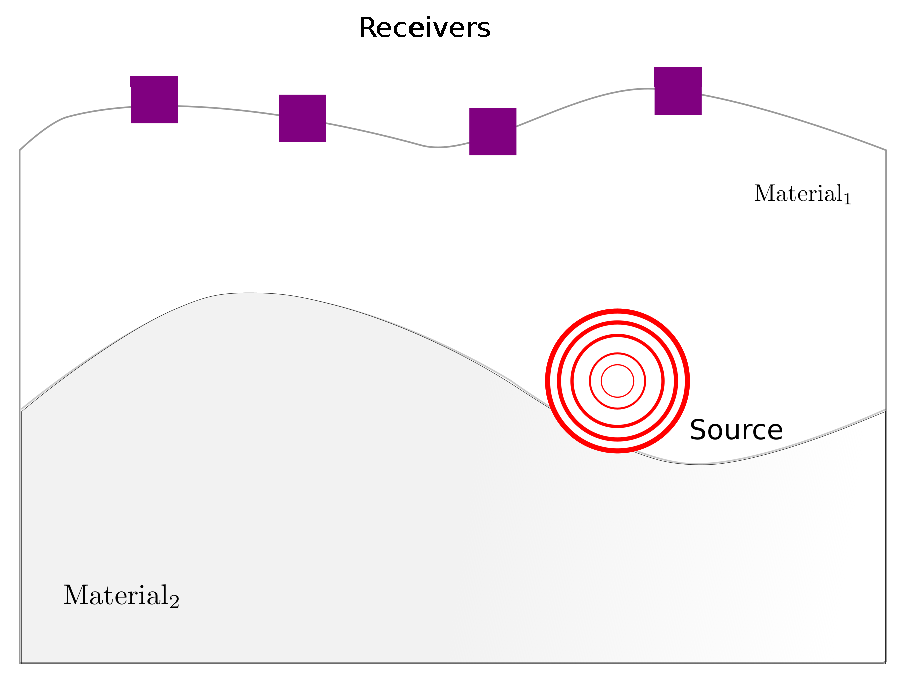
\includegraphics[width=0.5\linewidth]{setup}
	\caption{Experimental setup of the problem. An earthquake generated at source travels through material properties and the displacement of the earth is recorded at the receivers (purple squares). Based on the recording data of the receivers, we employ MCMC techniques to recover the source location. }
	\label{fig:setup}
\end{figure}

\subsubsection{Forward Problem}

We follow the analysis presented  in \cite{ motamed2013stochastic, motamed2015analysis,kocher2014variational,joly2003variational}. We denote the spatial variable by $\xx$ and the set of unknown parameters by $\te$. Consider an elastic,  non-homogeneous medium in an open, bounded set  $D\subset \R^d$, with $\partial D=\Gamma_D\cup \Gamma_N$, $\Gamma_D\cap \Gamma_N=\emptyset$, $|\Gamma_D|,\ |\Gamma_N|>0$, for $d=2,3$ and a time interval $I=[0,T]$. Given some complete probability space $(\Omega,F,P)$, \color{red} where $\Omega$ is...\color{black} we can pose the following stochastic initial boundary value problem given by \begin{subequations}\label{strongform}
	\begin{align}
	&\varrho(\xx,\te)\uu_{tt}(t,\xx,\te)-\del\cdot\mathbf{\sig}(\uu(t,\xx,\te))=\ff(t,\xx,\te) & \text{in } I\times D\times \Omega\\
	&\uu(0,\xx,\te)=\mathbf{g_1}(\xx), \ \ \uu_t(0,x,\te)=\mathbf{g}_2(\xx) & \text{on } \times D\times \Omega\\
	&\sig(\uu(t,\xx,\te))\cdot\mathbf{n}=\mathbf{0}& \text{on }I\times\Gamma_N\times \Omega,\\
	&\uu(t,\xx,\te)=\bm{0}&\text{ on } I\times\Gamma_D\times \Omega,
	\end{align}
\end{subequations}
where  $\uu: I\times D\times\Omega  \rightarrow\R^d$ $,\xx\in \R^d,\te\in\Omega, t\in I$, and with  $\sig=\lambda(\xx,\te)\del\cdot\uu I +\mu(\xx,\te)(\del\uu+(\del\uu)^T)$. Here we denote by $\uu$  the displacement vector, by $\varrho>0$ the material density, by $\lambda,\mu$ the Lam\'e parameters,  and by $\ff$ a (generalized) body force. \begin{assumption}\label{as:th} \color{red} include comment on assumptions\color{black}
	Let $s\geq 0$ be an integer. We assume that \begin{eqnarray}
	\ff(\cdot,\cdot,\te)\in\LL^2([0,T];\HH^s(D))\text{ for a.e. $\te\in \Omega$}, & \mathbf{g}_1\in \HH^{s+1}(D), &\mathbf{g}_2\in \mathbf{H}^s(D), \ \ s\geq 0.
	\end{eqnarray}
\end{assumption}
\noindent Under Assumption \ref{as:th}, problem (\ref{strongform}) admits a unique solution for a.e $\te \in \Omega$. We can then interpret the solution $\uu(t,\xx,\te)$ as a Banach space-valued function on $\Omega$  \cite{motamed2015analysis}, \begin{equation}\label{eq:wf_s}
\uu=\uu(\te):\Omega\rightarrow\bf{V}:=\mathbf{C}^0([0,T];\HH^{s+1}(D))\cap\mathbf{C}^1([0,T];\HH^s(D))\cap\HH^{2}([0,T];\HH^{s-1}(D)), \ \ s\geq 0.
\end{equation}
In turn, (\ref{eq:wf_s}) is a weak solution to problem (\ref{strongform}) provided that at $t=0$, $\uu(\te)=\mathbf{g}_1,\ \uu_t(\te)=\mathbf{g}_2$ and that for all test functions $\vv\in \mathbf{C}_0^\infty([0,T];H^1(D))$ the following weak formulation holds \begin{eqnarray}
\int_0^T\int_{D}\left(\varrho \uu_{tt}\cdot\vv+\del\vv:\sig(\uu)\right)d\xx dt=\int_0^T\int_{ D}\ff\cdot\vv d\xx dt.
\end{eqnarray}
For the analysis of the well possedness of the Bayesian inverse problem we will need $\uu$ to be Lipschitz in $\Omega$. To this end, we \color{red} quote,recall,...\color{black} the following theorem, presented in \cite{motamed2015analysis}:
\begin{theorem}\label{thm:lips} For the solution of problem (\ref{strongform}) with data given by Assumption \ref{as:th}  \color{red} check on additional assumptions on Motamed's paper \color{black} and with uniformly elliptic material properties,  we have that
	\begin{equation}
	\partial_{\theta_n}\uu(\te)\in\mathbf{C}^0([0,T];\HH^{s}(D)), \ \ s\geq 0,
	\end{equation}
	where $\theta_n$ denotes the $n^\text{th}$ component of $\te$. Moreover, $	\partial_{\theta_n}\uu(\te)$ is uniformly bounded in $\Omega$.
\end{theorem}
\begin{proof}
	The previous theorem is a particular case of Theorem 3 in \cite{motamed2015analysis}, for the case $k=1, $  \color{red} what is k?\color{black}and $s\geq 0$. 
\end{proof}
\begin{corollary}
	Under the assumptions of the previous theorem, $\uu(\te)$ is Lipschitz continuous, when seen as a map from $\Omega$ tp $\mathbf{C}^0([0,T];\HH^{s}(D))$.
\end{corollary}
\noindent For the purpose of this project, system (\ref{strongform}) is approximated numerically, using a spectral element method for the space discretization and the leapfrog method for the time marching scheme. 
\subsubsection{Observation Operator}
for the application at hand, data is gathered using an observation operator. As such, we will also need to study the properties of this operator in order to properly formulate the well possedness of the BIP.  We define the forward map $\fo:\Omega\rightarrow\R^{m\times N_{rec}}$ by  $$\bm{\mathcal{F}(\te)}=(\mathcal{O}_1(\uu(\te)),\dots,\mathcal{O}_{N_{rec}}(\uu(\te)),$$ where $\mathcal{O}_i\in(\mathbf{V}')^m$ is a linear observation operator at times $\{t_1,\dots,t_m \},$ associated to the $i^\text{th}$ receiver. In many problems in seismic inversion, data is only available at discrete points in the spatial domain, which in turn implies that the observation operator lacks enough regularity. To alleviate this, we define our $i^\text{th}$ linear operator as \begin{align}
\mathcal{O}_i(\vv)=\left(\frac{1}{|\mathcal{B}(\xx_i,r)|}\int_{{\mathcal{B}(\xx_i,r)}}\vv(t_1,\xx),\dots,\frac{1}{|\mathcal{B}(\xx_i,r)|}\int_{{\mathcal{B}(\xx_i,r)}}\vv(t_m,\xx)\right)^T,
\end{align} for any $\vv\in C^0([0,T],L^2(D))$, and where $\mathcal{B}(\xx_i,r)$ denotes the ball centered at $\xx_i$ with radius $r$. Let us denote $$\lv \fo (\te)\rv^2=\sum_{i=1}^{N_{rec}}\max_j\lv\mathcal{O}_{i,j}(\uu(\te))\rv^2.$$ 
% $$\Omega \ni\te\rightarrow\mathcal{F}:=(\mathcal{O}_1(\te),\mathcal{O}_2(\te),\dots,\mathcal{O}_{N_\text{obs}}(\te))=(\mathcal{O}_1(\uu(\te)),\mathcal{O}_2(\uu(\te)),\dots,\mathcal{O}_{N_\text{obs}}(\uu(\te))).$$ Here $V^*$ can be, for example \begin{align}
%V^*&=V_1=\LL^2([0,T];\HH^1(D))\cap \HH^1([0,T];\LL^2(D)), \quad \text{ or }\\
%V^*&=V_2=\mathbf{C}^0([0,T];\HH^1(D))\cap \mathbf{C}^1([0,T];\LL^2(D)).
Based on this, we can show that $\fo$ is Lipschitz continuous:
\begin{proposition}\label{prop:bdd_obs} Under the assumption of uniform ellipticity \color{red} define this or state as an assumption\color{black} on the material properties, $\bm{\mathcal{F}}$ is Lipschitz continuous. 	
\end{proposition} \color{red} not too happy with how equation is being displayed\color{black}
\begin{proof}
	We begin by noting that \begin{align}&| \mathcal{O}_{i,j}(\vv)|=
	\lv \frac{1}{|\mathcal{B}(\xx_i,r)|}\int_{\mathcal{B}(\xx_i,r)} \vv(t_j,\xx)d\xx\rv\nonumber \\&\leq \sqrt{ \frac{1}{|\mathcal{B}(\xx_i,r)|}\lno \vv(t_j,\cdot)\rno^2_{L^2(\mathcal{B}(\xx_i,r))}  }\leq \sqrt{ \frac{1}{|\mathcal{B}(\xx_i,r)|}\lno \vv(\te)\rno^2_{C^0([0,T];L^2(\mathcal{B}(\xx_i,r)))}}
	\end{align}
	 This in turn implies that  $\forall\  \te,\te'\in\Omega$, $$|\eff(\te)-\eff(\te')|\leq \Vert \uu(\te)-\uu(\te')\Vert_V.$$
Moreover, by Theorem \ref{thm:lips}, we have that there exist a $C_L>0$ such that $$\Vert \uu(\te)-\uu(\te')\Vert_V\leq C_L\Vert \te-\te'\Vert_{L^2(\Omega)},$$
thus, 
$$ |\eff(\te)-\eff(\te')|\leq C_L\Vert \te-\te'\Vert_{L^2(\Omega)}.$$\end{proof}
\subsubsection{Bayesian Formulation}
We consider a bounded and finite parameter space $\Omega$ \color{red} explain with bounded.\color{black} We will use the assumption of additive noise, i.e, we consider the case where we are given data $y$ polluted by some noise $\eta$, with $\eta,y\in \R^q$ and modeled by some forward map or linear observation operator $\mathcal{F}:\Omega\rightarrow\R^q$ such that
\begin{align}
y=\mathcal{F}(\te)+\eta, \quad \eta\sim g,
\end{align}
 where $f$ is some arbitrary probability distribution. Given the noisy, recorded data $y$, we are interested in determining a set of parameters $\te$ such that when used as input in $\ref{strongform}$, we obtain a wave form that closely resembles the one observed. To do so, we adopt a    Bayesian approach to the problem of determining $\te$ from $y$.  Roughly speaking, contrary to the deterministic counterpart, where only point estimates are obtained, the
Bayesian approach will lead to the notion of finding a probability measure
$\pi^y$ in $\Omega$, containing information about the relative probability of different
states $\te$, given the data y. Incorporating our prior beliefs in a density $\pi^0$ and denoting the conditional probability of $\te$ given $y$, by $\pi^y$, we have that from Bayes theorem \begin{align}
\pi^y\propto g(y-\mathcal{F}(\te))\pi^0(\te),
\end{align}
Moreover, we choose priors $\pi^0$ such that $\pi(\Omega)=1$, that is, the posterior is absolutely continuous with respect to the prior. Using Theorem 6.31 in \cite{stuart2010inverse}, we can rewrite the previous expression in terms of the Radon-Nikodym derivative \begin{align}\label{eq:radon}
\frac{d\pi^y}{d\pi^0}\propto\exp(-\Phi(\theta,y)),
\end{align}
where we are abusing notation and representing both density and distribution with the symbol $\pi$, and where we call $\Phi(\te,y)$ the potential function. For simplicity, we will limit ourselves to the case of additive Gaussian noise case; $$g=\mathcal{N}(0,\Sigma).$$



\newpage
\hspace*{0.3cm}
\color{red}  ALMOST FINAL DRAFT; DON'T KNOW IF I SHOULD INCLUDE A BRIEF DESCRIPTION OF MCMC \color{black}
\section{State of the Art}\label{sec::obj}
% 2.	Objectifs / Objectives: ½ page

\hspace*{0.3cm}

We now discuss the current state of the art of the research at hand. There are wo main points to address in this respect, the first one addresses the current state of seismic source inversion, and the second one addresses the state of  multi-level and multi-index Markov chain Monte Carlo methods. We begin by discussing the state of seismic inversion.

 
 \subsection{Deterministic Inversion}
 Traditionally, seismic inversion has been done using a deterministic approach; in the sense that a misfit function, measuring the differences in displacement or arrival time, is defined and then a parameter that minimizes this misfit is obtain using standard minimization algorithms, such as BFGS or conjugate gradient. This has been an approach used in numerous case studies, such as those presented in 
 \cite{epanomeritakis2008newton,krebs2009fast,hormander1985analysis} given the inherent computational
 \subsection{Probabilistic Inversion}
 One of the main drawbacks of the deterministic approach is 

 \subsection{Multilevel and Multiindex Monte Carlo}
\subsection{Mutilevel and Multiindex Markov Chain Monte Carlo}
Only few works so far have dealt with Multi-Level extensions of MCMC algorithms for posterior
exploration in Bayesian inversion [36, 37]. They both address the case of parameter identification for
elliptic PDEs and propose different strategies to build Multi-Level Metropolis-Hastings algorithms. We
will investigate improved versions of these MLMCMC algorithms and study their convergence proper-
ties in the context of parameter and/or source identification for second order hyperbolic problems (wave
equations), which are the underlying models in seismic applications. Moreover, the ideas in [36, 83,
84, 86, 87] on the construction of proposals for Metropolis-Hastings schemes, which are well defined
on function spaces, will be extended here to the case of spatially or temporally distributed parameters /
sources in the context of MLMCMC.
Finally, we will extend the Multi-Index framework described above in Section 1.3.1 to the MCMC
context. This sub-task concerns developing the MIMCMC algorithm and performing convergence ana-
lysis, as well as illustrating the results on problems of hyperbolic type. This task is specially challenging
given the limited regularity available in the hyperbolic problem. We note in passing that this task is
strongly related to the task T3.1 and indeed the expertise gained in one of the two tasks will be immedi-
ately applied in the other task.
\newpage

\hspace*{0.3cm}
\color{red}  WAITING FOR SOME RESULTS FROM THE CLUSTER, WILL UPDATE SOON  \color{black}
\section{State of Our Research and First Results}
% 3.	Premiers résultats / First results: 1-2 pages
We have focused mainly on three topics that tackle the problem at hand, both theoretically and computationally. More precisely, \begin{itemize}
	\item[i] We have studied and proved the well possedness of the BIP for the hyperbolic equation PDE at hand,
	\item[ii] We have implemented different sampling strategies to a case study inversion problem. These methods include random walk  Metropolis (RWM), adaptive Metropolis, delayed rejection adaptive metropolis (DRAM), and parallel tempering. 
	\item[iii] We have proposed a MLMCMC algorithm and tried different sampling strategies. 
	\end{itemize}
 In addition, we have also started to look  into other research directions which shall be discussed in Section 4. We proceed to discuss in more detail the three points explained above. 
\subsection{On the Well-Possedness of the BIP}
We mention the results pertaining the well possedness of the BIP.  The results shown herein are an extension to \cite{stuart2010inverse,hoang2013complexity,dodwell2015hierarchical}, and can be found in more detail in the upcoming work \cite{Madrigal2018ssi}. For simplicity, we omit most of the proofs relating to the minor results.
\begin{definition}
	Let $\mu,\ \nu$ be two distributions with Radon-Nikodym derivative with respect to a common measure $\lambda$ given by $\frac{d\mu}{d\lambda},\ \frac{d\nu}{d\lambda},$ respectively. The Hellinger distance between $\mu$ and $\nu$ is defined as \begin{align}
	d^2_\text{Hell}(\mu,\nu)=\int_X\left(\sqrt{\frac{d\nu}{d\lambda}}-\sqrt{\frac{d\mu}{d\lambda}}\right)^2d\lambda.
	\end{align}
\end{definition}	
\noindent Notice that the Hellinger distance is ralated to the total variation (TV) norm by $$d^2_\text{Hell}(\mu,\nu)\leq d_\text{TV}(\mu,\nu)\leq \sqrt{2}d_\text{Hell}(\mu,\nu),$$ which follows from the relationship between the 1 and 2 norms.
\begin{proposition}
Let $\te\in\Omega$, where $\Omega$ is a bounded domain. Moreover, Assume that for each component of $\te$, $0<\te^i_{\min}\leq\te^i\leq \te^i_{\max}<\infty$. Then $\uu(\te)$ is uniformly bounded in $\Omega$. 
\end{proposition}\noindent The proof of the preceding theorem can be found in \cite{motamed2015analysis}.\\
\\
%\begin{assumption}\label{as_phi}
%	Let $X,Y$ be some separable Banach spaces such that $\te\in X, y\in Y$. $\Phi(\te;y):X\times Y\rightarrow\R$ has the following properties:\begin{enumerate}
%		\item $\forall \epsilon,r>0,\exists M(\epsilon,r)>0$ such that $\forall\te\in X , y\in Y $, $\Vert y\Vert_Y<r, $ $$\Phi(\te;y)>M-\epsilon\Vert \te \Vert^2_X,$$\
%		that is, there is a lower bound on the potential function.\label{ap1}
%		\item $\forall r>0, \exists K(r)>0$ measurable such that $\forall \te\in X,\ y\in Y$, with $\max\{	\Vert\te\Vert_X,\Vert y\Vert_Y		\}<r,$ $$\Phi(\te;y)\leq K(r),$$
%		i.e, there is an upper bound on the potential.\label{ap2}
%		\item $\forall r>0, \exists L(r)>0$ such that $\forall \te, \te'\in X, y\in Y $, with $\max\{ \Vert\te\Vert_X, \Vert\te'\Vert_X,\Vert y \Vert_Y\}<r, $ $$\vert \Phi(\te;y)-\Phi(\te';y)\vert \leq L(r) \Vert \te-\te'\Vert,$$ which means that we have Lipschitz continuity of $\Phi(\cdot; y) $ with respect to $\te$. \label{ap3}
%		\item $\forall \epsilon,r>0,\ \exists C(\epsilon,r)>0\in \R, $ such that $\forall y_1,y_2\in Y, \te in X, $ with $\max \{	\Vert y_1\Vert_Y, \Vert y_2\Vert_Y		\}<r, $ $$\vert \Phi(\te;y_1)-\Phi(\te;y_2)\vert\leq \exp(\epsilon \Vert\te\vert^2_X+C)\Vert y_1-y_2\Vert_Y$$\label{ap4}
%	\end{enumerate}
%\end{assumption}
\noindent Given a covariance matrix $\Sigma$, we define the potential function (i.e, the negative log-likelihood) $\Phi(\te;y)$ by  \begin{equation}\label{pot}
\Phi(\te;y)=\frac{1}{2}\vert y-\mathcal{F}(\te)|^2_{\Sigma^{-1}}.
\end{equation} Analogously, we define the potential arising from a discretized PDE with discretization parameter $h_\ell$ by $\Phi_{\ell}(\te;y)$.
% \begin{assumption}\label{as2}
%	
%	\begin{enumerate}
%		\item[i)] Given $\epsilon>0,\ \exists\  M(\epsilon)\in \R$ such that  $ \forall \te\in X$, $$\vert \mathcal{F}(\te)\vert_\Sigma\leq \exp(\epsilon\Vert \te \Vert^2_X+M).$$\\
%		\item[ii)] $\forall r>0, \exists K(r)>0$ measurable in $X$, such that $\forall \te, \te'$, with $\max\{ \Vert\te\Vert_x,	\Vert\te'\Vert_x,			\}<r, $ $$\vert \mathcal{F}(\te)-\mathcal{F}(\te')\vert_\Sigma\leq K\Vert \te-\te'\Vert_X.$$
%	\end{enumerate}
%\end{assumption}
%\noindent Notice that Assumptions \ref{as2} are satisfied since we have that $\uuh$ is uniformly bounded in $\Omega$. 
%\begin{proposition}
%	Under the assumption of a finite dimensional space and a continuous potential function of the form (\ref{pot}), if the assumptions \ref{as2} are satisfied, so are the assumptions in \ref{as_phi}.
%\end{proposition}
\begin{proposition} We have that, for each level $\ell$, the potential function is locally bounded, i.e, there exists $\Phi^M(r)$ such that $$0\leq \Phi_{\ell}(\te;y)\leq\Phi_\ell^M(r).$$ Additionally, this potential function is locally Lipschitz with respect to both the data $y$ and the parameter $\te$, i.e, there is a mapping $G: \R\times \te \rightarrow \R$ and a constant $C_\text{pot}$ such that for each $r > 0$, $G(r, \cdot) \in L^2(\te)$; and for every $|y|,|y'|$, it holds that \begin{equation}\label{lip_in_y}\vert \Phi_{\ell}(\te;y)-\Phi_{\ell}(\te;y')\vert\leq G(r,\te)|y-y'|_{\Sigma^{-1}},\end{equation} and
\begin{equation} \label{lip_in_te}\vert \Phi_{\ell}(\te;y)-\Phi_{\ell}(\te';y)\vert\leq C_\text{pot}\Vert \te -\te'\Vert_{L^2(\Omega)}. \end{equation}
\end{proposition}
\begin{proposition}
	For each positive constant $r$ there is a positive constant $C(r)$ such that if $|y|_\Sigma,|y|_\Sigma\leq r$, then $$d_\text{Hell} (\pi^y,\pi^{y'})\leq C(r)|y-y'|_\Sigma.$$
\end{proposition} 

\begin{proof}
	The proof follows from that of proposition 25 in \cite{hoang2013complexity}. %We let $Y=(\R^n,\Vert\cdot\Vert=|\cdot\Sigma^{-1/2}\cdot|)$. Assumption \ref{ap2}(2) implies that there exists a measurable $K(r)$ that only depends on $r$, such that $\Phi(\te;y)\leq K(r)$. We denote the normalizing constant of $\pi^y$ as $z^y=\int_\Omega\exp(-\pot)d\pi^0(\Omega)$. Since $\pot\geq 0\forall \te \in \Omega$ (given that it is well defined), this we have that  \begin{equation}z^y=\int_\Omega \exp(-\pot)d\pi^0(\Omega)\geq\int_\Omega K(r)d\pi^0(\Omega)=K(r)\pi^0(\Omega).\end{equation} On the other hand, given that for $v,w\geq 0$, $|\exp(-w)-\exp(-v)|\leq |w-v|$, we have that \begin{equation}
%	|z^y-z^{y'}|=\vert \int_\Omega (\exp(-\pot)-\exp(\potp))d\pi^0\vert\leq \int_\Omega|\pot-\potp|d\pi^0\leq C(r)\vert y-y'\vert_\Sigma,
%	\end{equation}
%	where we used Assumption \ref{ap3}(3), and the fact that the constant therein is implied to be integrable in $\Omega$, i.e, $C(r)$ takes the form $\exp(\epsilon \Vert \te\Vert_\Omega^2+C')\pi^0(\Omega)$. Thus, \begin{align}|z^y-z^{y'}|\leq C(r)\vert y-y'\vert_\Sigma.\end{align}
%	Moreover, we have that given the properties of the Hellinger distance $$2\dhell(\pi^y,\pi^{y'})\leq I+II,$$ with \begin{align}
%	I&=\frac{2}{z^y}\int_\Omega\left (\exp(-\frac{1}{2}\pot)-\exp(-\frac{1}{2}\potp)\right)^2d\pi^0,\\
%	II&=2|(z^y)^{-1/2}-(z^{y'})^{-1/2}|^2\int_\Omega\exp(-\potp)d\pi^0.
%	\end{align}
%	From the same arguments as before, $I\leq K(r)\vert y-y'\vert$. Moreover, $$|(z^y)^{-1/2}-(z^{y'})^{-1/2}|^2\leq K(r)\vert z^y-z^{y'}\vert \leq K(r)\vert y-y'\vert_\Sigma,$$
%	which proves the proposition.
%	This, in turn is equivalent to proposition 3 in \cite{hoang2013complexity}, which gives the well-possedness of the Bayesian Posterior.
\end{proof}

\begin{theorem}
Under the preceding propositions, the Bayesian inverse problem is well posed. 
\end{theorem}
\color{red} Waiting for some results, need to update the problem description here, as well as including pictures on the domain, etc. I have some older ones that I obtained with the desktop pc, but I re-run the experiments in the cluster.  \color{black}
\subsection{Solving the Inverse Problem: The Tanzania Case Study}
We now address the results claimed in (ii). In particular, we implemented different MCMC algorithms and applied them to a simplified seismic source inversion problem. More precisely, we test the data on a  2-dimensional model of an earthquake that took place on the Tanzania basin on the 12th of October 2016 at 1:31:53\footnote{Other source inversion experiments using this case study are currently being run by other recipients of the KAUST CRG4 grant.}. We are interested in locating the spatial component of the source of an earthquake. Moreover, we consider the material properties of the ground $\rho,\mu,\lambda$ to be uncertain. However, we claim to know some of the structure of the medium, such as layer position. The experiment are run for $T=17$, $\Delta t=10^{-3}$, on a mesh of $58\times34$ elements. The spatial part of the wave equation is discretized using a spectral element method with 5 Gauss-Legendre-Lobatto (GLL) nodes per element, and the time marching scheme is done using a leapfrog method.  In particular we compare random-walk Metropolis (RWM), delayed rejection adaptive Metropolis (DRAM),  and Parallel-Tempering (PT).
\begin{figure}
	\centering
	\begin{subfigure}[a]{0.4\textwidth}
	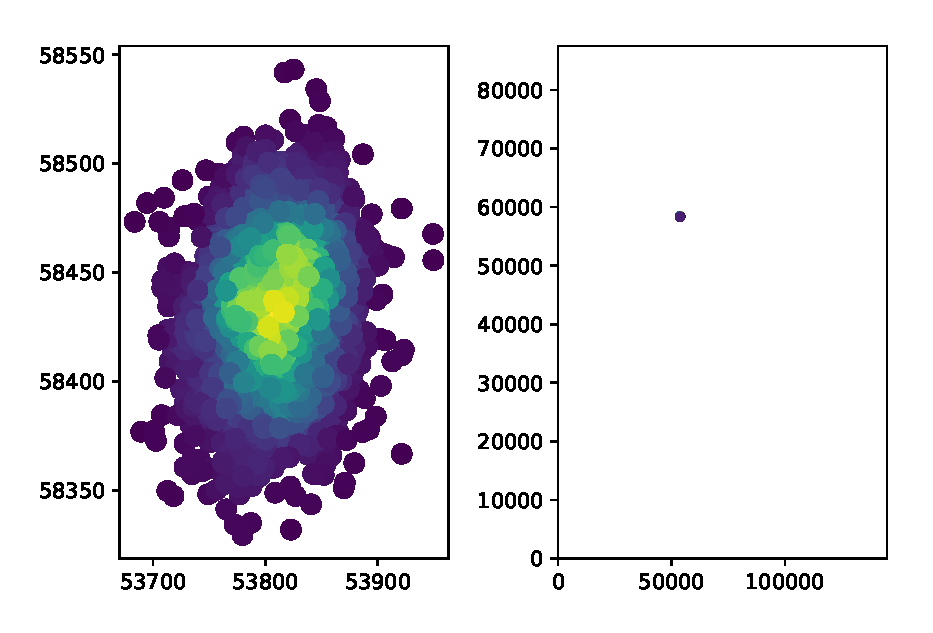
\includegraphics[width=\textwidth]{figures/dens}
		\label{fig:dens}
	\caption{Here we can see the probability density for the spatial components of the source location. The left figure is a zommed-in version of the right one. }
	\end{subfigure}
	\begin{subfigure}[b]{0.4\textwidth}
	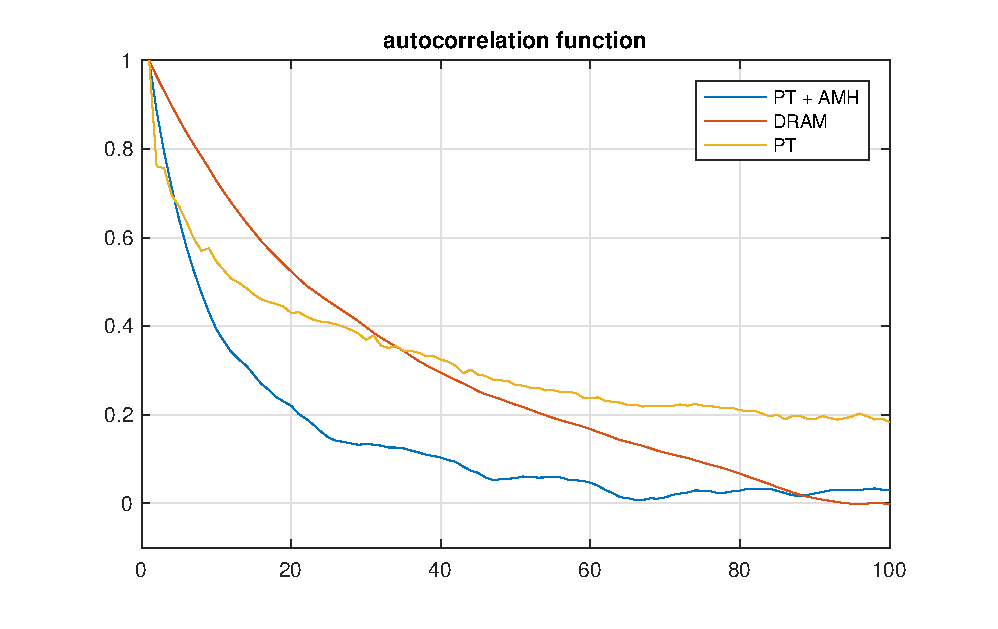
\includegraphics[width=\textwidth]{figures/acf_tanz}
		\label{fig:acf}
		\caption{Autocorrelation function for different samplers. As we can see, the most efficient sampler is the combination of parallel tempering and adaptive Metropolis. All samplers took equivalent time.  }
	\end{subfigure}
	\caption{Inversion Results}\label{fig:animals}
\end{figure}

\color{red} same as before, I have some older results on the toy problem with the KDE and some results for a toy problem using the ideal proposal (sampling for normals), but I guess including upcoming results might be better.\color{black}
\subsection{MLMCMC strategy}






\hspace*{0.3cm}
Only few works so far have dealt with Multi-level extensions of MCMC algorithms for posterior exploration in Bayesian inversion (\cite{hoang2013complexity} \cite{dodwell2015hierarchical}). Both authors address the case of parameter identification for elliptic PDEs and propose different strategies in order to build Multi-Level Metropolis-Hastings algorithms. 
%\begin{enumerate}
%	\item borrows  ideas form mlmc\dots,
%	\item introduce a hierarchy of meshes $h_\ell$, $\ell=0,\dots, L$, to which there will correspond a a posterior $\pi_\ell$ and a number of samples $N_\ell$.  
%	\item We diverge from the notation of the \cite{hoang2013complexity}, in the sense that we do not consider two different discretizations for the solution and the posterior. Moreover, we assume that we are on a finite parameter space, and as such, we don't need to introduce a mode discretization, as it is done in \cite{dodwell2015hierarchical}
%\end{enumerate}
As for multigrid methods applied to discretised (deterministic) PDEs, the key is to avoid estimating
the expected value of $Q_\ell$ directly on level $\ell$, but instead to estimate the correction with respect to the
next lower level. Since in the context of MCMC simulations, the target distribution $\pi$
depends on the discretization parameter $\ell$,
the new multilevel MCMC (MLMCMC) estimator has to be defined carefully \cite{dodwell2015hierarchical}. We will use the identity
$$\E_L=\sum_{\ell=0}^{L}\E_{\ell}[Q_\ell]-\E_{\ell-1}[Q_{\ell-1}],$$ where $Q$ is some quantity of interest and where we have used the convention that $\ell=-1$ means the expectation w.r.t the 0 measure. We define the increments $Y_\ell=Q_\ell-Q_{\ell-1}$. There are two main ideas  underlying the reduction in computational cost associated with
the multilevel estimator: \begin{itemize}
	\item Samples at level $\ell$ are cheaper to estimate
	\item The Variance of $Y_\ell$ goes to 0 as $\ell$ goes to infinity.
\end{itemize}
To guarantee the reduction in computation effort, we use the following assumptions:
\begin{assumption}\label{mlmcmc:assumptions}The following are assumed to hold:
	\begin{enumerate}
		\item $\exists \alpha>0$ such that $\Vert \uu-\uu_{h_\ell}\Vert_V\leq C_1h^{-\alpha \ell}$, where $u_\ell$ denotes the solution with discretization parameter $h_\ell$.
		\item $\exists \beta>0$ such that $\V_\ell[ Y_\ell] \leq C_2h^{-\beta \ell}$, where $u_\ell$ denotes the solution with discretization parameter $h_\ell$; $Y$ defined to be the increment as in \cite{dodwell2015hierarchical}.
		\item $\exists \gamma>0$ such that the cost $\mathcal{C}_\ell$ associated to evaluating $\pot_\ell$ behaves as $\mathcal{C}_{\ell}\leq C_3h^{-\gamma}$.
		\item We can generate samples from $\pi_\ell, \pi_{\ell-1}$ using an independent sampler MH algorithm.
	\end{enumerate}
\end{assumption}
\begin{center}
	Notice that $1$ and $3$ in Assumption \ref{mlmcmc:assumptions} are related to the PDE at hand. An algorithm that 
	\fbox{\begin{minipage}{35em}
			\begin{algorithmic}[1]
				\Function{MLMCMC}{$\{N_\ell\}_{\ell=0}^L,\{\pi_\ell\}_{\ell=0}^L,q,\theta^0$}
				\If {$\ell=0$}
				\State $\chi_{0,0}=$\texttt{Metropolis-Hastings}($N_0,\pi_0,q,\theta^0$)
				\EndIf
				\For{$\ell=1,\dots,L$}
				%\State Approximate $\pi_{\ell-1}$ by $\hat{\pi}_{\ell-1}$.
				\For {$n=1,2,\dots,N_\ell-1$}
				\State Sample $\tilde{\theta}\sim\hat{\pi}_{\ell-1} $.
				\State Set $\theta^*\sim q(\tilde{\theta})$.
				\For{$j=\ell-1,\ell$}
				\State Set $\theta_{\ell,j}^{n+1}=\theta^*$ with acceptance probability $\alpha_j$:
				$$\alpha_j(\theta_{\ell,j}^n,\theta^*)=\min \left[\frac{\pi_j(\theta^*)q(\theta_{\ell,j}^{n})\hat{\pi}_{\ell-1}(\theta_{\ell,j}^n)}{\pi_j(\theta_{\ell,j}^n)q(\theta^*)\hat{\pi}_{\ell-1}(\theta^*)},1\right].$$
				\State Set $\theta_{\ell,j}^{n+1}=\theta^n$ otherwise.
				\EndFor
				\EndFor
				\State Create chains $\chi_{\ell,\ell-1}=\{\theta_{\ell,\ell-1}^n\}_{n=0}^{N_\ell}$ and $\chi_{\ell,\ell}=\{\theta_{\ell,\ell}^n\}_{n=0}^{N_\ell}$
				\EndFor
				\State Output $\chi_{\ell,\ell},$ and $\chi_{\ell,\ell-1}$ for $\ell=0,\dots,L$.
				\EndFunction
			\end{algorithmic}
	\end{minipage}}
\end{center}
Note that in the case where we generate proposals by subsampling from the previous chain we obtain the algorithm presented in \cite{dodwell2015hierarchical}. We present some definitions that we will use throughout the rest of the paper.
\begin{definition}
	We say that at a given level $\ell$ and iteration $n$, the chain \textbf{diverged} if $\te^n_{\ell,\ell}\neq \te^n_{\ell,\ell-1}$.
\end{definition}
\subsection{On how to generate $\hat{\pi}_\ell$}
\noindent One thing that has not been discussed so far is how to choose $\hat{\pi}_{\ell}$. We now discuss some proposal generating functions for the independent sampler
\subsubsection{Ideal Proposal}
We first study the ideal, (yet no implementable for the majority of the problems), case for which we are able to do an independent sampler generating proposal from the target distribution at the previous level. That is, suppose that at each level $\ell$ , $\pi_\ell=\hat{\pi}_\ell$. Thus, given a sequence of target distributions $\{\pi_\ell\}_{\ell=1}^\infty$, we generate candidate states from $\pi_{\ell-1}$ at each iteration, i.e, we generate proposal states by $$\te^*\sim \pi_{\ell-1}.$$ Even if this \textit{oracle} algorithm is not implementable in practice for the majority of more \textit{ interesting}
problems, we can learn some of the properties that belong to the ``best case scenario" algorithm.
\begin{proposition}
	Let $\pi_{\ell-1}=\hat{\pi}_{\ell-1},$ and  let there be a $C_1$ such that $\pi_\ell\leq C_1\pi_{\ell-1}$. Then, assuming that we are on a bounded state space and that $\forall \te\in\Omega$ and $ \ell\geq0, $ we have that $\pi_\ell(\te)>0$, the following holds: \begin{enumerate}
		\item The acceptance rate $\alpha_\ell\rightarrow 1$ as $\ell\rightarrow\infty$. 
		\item The integrated autocorrelation time $\tau$ goes to 1  as $\ell\rightarrow\infty$, assuming that we can generate i.i.d samples from $\pim$.
	\end{enumerate}
%	\begin{proof}
%		Firstly, notice that for each level, the acceptance rate at the previous level $\ell-1$, is always 1 since $\hat{\pi}_{\ell-1}=\pi_{\ell-1}$. Thus:
%		$$a_{\ell-1}=\min\left[\frac{\pi_{\ell-1}(\theta^*)q(\theta_{\ell-1}^n)\pi_{\ell-1}(\theta^n)}{\pi_{\ell-1}(\theta^n)q(\theta_{\ell-1}^*)\pi_{\ell-1}(\theta^*)},1\right]=\min[1,1]=1.$$
%		This means, that the probability of diverging at any given iteration is $1-\alpha_\ell$. Thus, we have that the expected divergence at level $\ell$ is given by $$\E[1-\alpha_\ell]=1-\E[\alpha_\ell]\geq1-\frac{1}{C_1},$$
%		where Proposition \ref{prop3} was used in the inequality. Moreover, in an act of abbusive notation,  we denote $\pi_\ell,\pi_{\ell-1}$ the density of the distributions at both levels. Taking the difference of the distribution evaluated at $\te$, we obtain \begin{align}
%		|\pim-\pil|&=\left\vert \frac{e^{-\potm}}{Z_\ell}-\frac{e^{-\potl}}{Z_{\ell-1}}\right\vert \leq \left\vert \frac{e^{-\potl}}{Z_{\ell}} -\frac{e^{-\potl}}{Z_{\ell-1}}\right\vert +\left \vert \frac{e^{-\potm}}{\zm}-\frac{e^{-\potl}}{\zm} \right \vert \nonumber \\
%		&= \lv \frac{1}{\zm}\rv \lv e^{-\potm}-e^{-\potl}\rv+\lv \frac{e^{-\potl}}{\zl}\rv\lv1-\frac{\zl}{\zm}\rv \nonumber \\
%		&\leq \lno \uu_\ell-\uu_{\ell-1}\rno_X+\lv \frac{e^{-\potl}}{\zl}\rv \lv \frac{\zm-\zl}{\zl\zm}\rv \nonumber \\
%		&\leq \lv \frac{1}{\zl}\rv \left[  c_{\te} h^{\alpha\ell}+\frac{e^{\Phi(r)}}{|\zl\zm|}\lv\zm-\zl\rv \right].
%		\end{align}
%		Now, notice that $$\lv \zm-\zm\rv =\lv \int_\Omega e^{-\potm}-e^{-\potl}d\pi^0\rv\leq  \int_\Omega \lv e^{-\potm}-e^{-\potl}\rv d\pi^0,$$
%		Thus, we have that 
%		$$ \int_\Omega \lv e^{-\potm}-e^{-\potl}\rv d\pi^0\leq \int_\Omega \lv \uu_\ell -\uu_{\ell-1}\rv d\pi^0\leq C_{\te} h^{\alpha \ell }$$
%		Finally since $(1/C_1)\leq \pil/\pim$, we have that $$\left(1-\frac{1}{C_\ell}\right)\vert\pil\vert=\vert(1-\frac{1}{C_\ell})\pil\vert    \leq\vert \pil\left(1-\frac{\pim}{\pil}\right)\vert\leq  K_\ell(\te)h^{\alpha\ell},$$
%		and as such, $\E[\text{divergence}]\rightarrow 0$ as $\ell\rightarrow\infty$.
%		The second part is evident; under the assumption that we can generate iid samples from $\pi_{\ell-1}$, and since the acceptance rate tends to 1, then the autocorrelation of the samples at level $\ell$ will become 0. 
%	\end{proof}
%	
	
\end{proposition}	
\subsubsection{Sampling From the Prior}
\color{red}there is a result that quantifies the conv. rate for ind. sampler based on bounds of the lielihhod, i'll include it soon \color{black}
\subsubsection{KDE approximation}
One possible way of generating $\hat{\pi}_{\ell-1}$ is to create a KDE based on the samples obtained at the previous level. 
\subsubsection{Laplace's Approximation}
Alternatively , we can use Laplace's approximation in order to compute $\hat{\pi}_{\ell-1}$ under the assumptions that (i) it is a smooth function in $\Omega$ and (ii) that the distribution is well peaked. Under these assumptions, we have that, denoting $q_{\ell-1}(\te)=\hat{\pi}_{\ell-1}$ and  omitting the dependence on the level for notational clarity, the Taylor expansion of $q(\te)$ around is maximum a posteriori (MAP) $\te^{MAP}$ is given by 
\begin{align}
q(\te)&=q(\te')+(\te-\te^{MAP})^T\del q(\te)+\frac{1}{2}(\te-\te^{MAP})^TH(\te-\te^{MAP}) + \mathcal{O}((\te-\te^{MAP})^3) \nonumber,\\
&=q(\te')+\frac{1}{2}(\te-\te^{MAP})^TH(\te-\te^{MAP}) + \mathcal{O}((\te-\te^{MAP})^3), \ \ \text {since $\del q(\te^{MAP})=0$}\nonumber,\\
&\approx C-\frac{1}{2}(\te-\te^{MAP})^TH(\te-\te^{MAP}),
\end{align}
%	 	which can be interpreted as the logarithm of a normal distribution with variance $H$ (the Hessian) with mean $\te^{MAP}$. Moreover, it can be shown  \cite{schillings2018} that \begin{align}
%	 	d^2_{Hell}(\pi,\hat{\pi})\in \mathcal{O}
%	 	\end{align}  
Despite being an interesting approach and having some desirable properties (see \cite{schillings2018}), this approach has two main drawbacks. The first one is the lack of generality, as it is not always the case that a posterior has a unique maximizer. The second one is the computational challenge of computing the Hessian. This however, can be approximated and computed "in line" if an optimization algorithm is used to find the MAP. 
\subsubsection{Optimization of a Parametric Family}
An additional approach to computing $\hat{\pi}_{\ell-1}$ is as based on the minimization of the Hellinger distance between $\pi_{\ell-1}$ and $\hat{\pi}_{\ell-1}$. Formally, we seek to approximate ${\pi}_{\ell-1}$ using a parametric family of distributions with density  $f(\te;\gamma)$, where $\gamma$ is given by \begin{align}
\gamma^*=\min_{\gamma\in \Gamma}\int_\Omega \frac{1}{2}\left(\sqrt{\hat{\pi}_{\ell-1}}-\sqrt{f(\te;\gamma)}\right)^2d\gamma +\frac{\alpha}{2}R(\gamma),
\end{align}
where $R$ is a regularizer with regularization term $\alpha$.  Notice that the previous integral can be rewritten in terms of an expectation with respect to the samples of the previous  chain $\chi_{\ell-1,\ell-1}$ as \begin{align}
\E_{\pi_{\ell-1}}\left[ \left(\sqrt{{\pi}_{\ell-1}}-\sqrt{f(\te;\gamma)}\right)^2\frac{1}{{\pi}_{\ell-1}}	\right],
\end{align}
thus, the optimization problem can be read as find $\gamma^*$ such that
\begin{align}
\gamma^*=\min_{\gamma\in \Gamma}\ \ \E_{\pi_{\ell-1}}\left[ \left(\sqrt{{\pi}_{\ell-1}}-\sqrt{f(\te;\gamma)}\right)^2\frac{1}{{\pi}_{\ell-1}}	\right]+\frac{\alpha}{2}R(\gamma).
\end{align}
This expectation can in turn be approximated with error $N_\ell^{1/2}$ by 
\begin{align}
\approx\frac{1}{N_\ell}\sum_{i=1}^{N_\ell}\left[\left(\sqrt{{\pi}_{\ell-1}(\te^i)}-\sqrt{f(\te^i;\gamma)}\right)^2 {\pi}^{-1}_{\ell-1}(\te ^i )\right]+\frac{\alpha}{2}R(\gamma).
\end{align}
Moreover, note that it is possible to save the values of the un-normalized posterior $\pi_{\ell-1}$ at the previous level,  and as such, this optimization algorithm should represent a  lower cost with respect to the solution of the PDE. Moreover, note that each approximation can be improved at the next level, given that each chain is evaluated twice in the algorithm.  Alternatively, a similar approach can be proposed minimizing the Kullback-Lieber divergence.

%\noindent Notice that when using SEM (with $p\geq 1)$ with a regular grid, the discretization error is dominated by the time-error. Moreover, from the CFL condition we have that $h=\mathcal{O}(\dt)$, and as such, the ``worst case scenario" (for long time integration) we have that $\alpha =2$. A similar argument holds for assumption $(ii)$. Assumption $(iii) $ is shown in \dots, which is an adaptation for our case of proposition 5 in \cite{hoang2013complexity}. Assumption $(iv)$ follows trivially. 



\newpage
\hspace*{0.3cm}
\color{red} HALF-WAY DONE (wanted to try to include some experiments with the transport maps), but I wonder if I should move sections 3.4.2 to 3.4.5 here?  \color{black}
\section{Future planning}
% 4.	Planification future (plan de travail) / Future planning (scheme of work): ½ page
\begin{itemize}
\item There are some pictures here to be included soon \color{black}\\
\end{itemize}
\noindent There are different research directions and projects that would be nice to explore in the future, both from a computational and from a theoretical perspective. We here present an outline of the ideas that we would like to explore during the duration of this project. \\ \\ \noindent 
\begin{itemize}
	\item There are still many different ways of proposing MLMCMC algorithms, two of which have been discussed and will be studied in the near future. The first one is to extend the same framework of the parallel tempering algorithm, where multiple chains using different noise levels ( so called ``temperatures'') are run in parallel and set to exchange states using a Metropolis-Hastings acceptance-rejection step every so often, to a multi-level or even multi-index setting, where there would be temperatures and discretization levels to take into account. A similar idea to this has been implemented in the context of sequential Monte Carlo by \cite{latz2017multilevel}. 
	\item The other interesting research direction arises when combining multi-level ideas with transport maps. Transport maps have been studied in \cite{marzouk2016introduction,parno2016multiscale,parno2018transport} and used as an efficient way of accelerating  MCMC.\\ 
	\item Concerning the inversion problem, it would be interesting to move the project into more challenging problems, such as those involving Cartesian three dimensional models, or source inversion at a global scale. It is also important to apply the methods explored herein to inversion of slip faults, rather than ``just" point sources, as these represent more realistic models. 
	\item Concerning the inversion problem, it would be interesting to move the project into more challenging problems, such as those involving Cartesian three dimensional models, or source inversion at a global scale. It is also important to apply the methods explored herein to inversion of slip faults, rather than ``just" point sources, as these represent more realistic models. 
	\item We are interested in performing Bayesian inversion for the source location. However, in many cases the material properties of the earth are deemed to be uncertain, and as such can be treated as nuisance parameters in the Bayesian inversion.\color{red} this transition here can be done more smoothly \color{black} In more technical terms,  denoting by $\te^s, \te^e$ the  (unknown) source and material properties respectively, in such a way that $\te=(\te^s,\te^e)$, we would like to obtain $\pi(\te^s|y)$ based on $\pi(\te^s,\te^e|y)$. Thus, \begin{align}
\pi(\te^s|y)&=\int_{\Theta^e}\pi(\te^s,\te^e)\pi(\te^e)d\te^e \label{marg}\\ &\approx\frac{1}{N}\sum^N_{i=1}\pi(\te^s,\te^e_i), \quad \te^e\sim \pi(\te^e).\label{mcmarg}
	\end{align} We can therefore combine two ideas to obtain samples from $\pi(\te^s|y)$; we can use the pseudo-marginal MCMC  \cite{andrieu2009pseudo} to sample from  $\pi(\te^s|y)$ where we can only access $\pi(\te^s,\te^e|y)$, and, additionally, we can use a  multi-level Monte Carlo for a fast computation of the expected value (\ref{mcmarg}).  
	\item Lastly, it would be a very interesting idea to collect all these sampling strategies, multi-level or not, and implement a library  (either in MATLAB or python) that can be used as a ``blackbox'', so that other research groups can use the methods developed in this work. \\
\end{itemize}

\newpage
\color{red}  This is probably done  \color{black}
\hspace*{0.3cm}
\section{Miscellaneous}
%5.	Divers / Miscellaneous
%	5.1 Eventuelles publications / Publications
%	5.2 Présentation(s) orale(s) / Oral presentation(s)
%	5.3 Cours suivis / Courses attended



\subsection{Conferences}

\begin{itemize}
	\item Uncertainty quantification for complex systems: theory and methodologies, Isaac Newton Institute of Mathematical Sciences, Cambridge, UK., 09.03.18-15.03.18 \\ 
	\textit{Poster: Bayesian Approaches to a Seismic Source Inversion Problem.}

\end{itemize}

\subsection{Courses and Workshops Attended}

\begin{itemize}
	\item Gene Golub Summer School 2018: "Inverse Problems: Systematic Integration of Data with Models under
	Uncertainty." Breckenridge, Colorado. June 17-30, 2018 - \textit{(4 credits)}
	\item Nobile, Fabio, "Stochastic Simulations". Mathematics, MATH 414. EPFL - (\textit{5 credits})
	\item SpeedUp Workshop, University of Bern.
	\item Parallel computing mini-classes at EPFL (offered by SCITAS).
	
\end{itemize}

\subsection{Others}

\begin{itemize}
	\item Academic Visit, King Abdullah University of Science and Technology, from 11.17-12.17 and 16.03.18-06.04.18. Stochastic Numerics Research Group, in charge of Prof. Ra\'ul Tempone. 
	\item Co-supervisor of Master thesis, Marc  Witkowski \textit{Monte Carlo Methods For Contact Problems with Rough Surfaces}. February 2018.
	\item Co-supervisor of Master thesis, Mathieu Odobez. \textit{The Zig-Zag Method for Inversion Problems}. July 2018.

\end{itemize}



\hspace*{0.3cm}

\newpage
\nocite{*}
\bibliography{bib}
\bibliographystyle{plain}
\newpage



\end{document}  